% Template for Cogsci submission with R Markdown

% Stuff changed from original Markdown PLOS Template
\documentclass[10pt, letterpaper]{article}

\usepackage{cogsci}
\usepackage{pslatex}
\usepackage{float}
\usepackage{caption}

% amsmath package, useful for mathematical formulas
\usepackage{amsmath}

% amssymb package, useful for mathematical symbols
\usepackage{amssymb}

% hyperref package, useful for hyperlinks
\usepackage{hyperref}

% graphicx package, useful for including eps and pdf graphics
% include graphics with the command \includegraphics
\usepackage{graphicx}

% Sweave(-like)
\usepackage{fancyvrb}
\DefineVerbatimEnvironment{Sinput}{Verbatim}{fontshape=sl}
\DefineVerbatimEnvironment{Soutput}{Verbatim}{}
\DefineVerbatimEnvironment{Scode}{Verbatim}{fontshape=sl}
\newenvironment{Schunk}{}{}
\DefineVerbatimEnvironment{Code}{Verbatim}{}
\DefineVerbatimEnvironment{CodeInput}{Verbatim}{fontshape=sl}
\DefineVerbatimEnvironment{CodeOutput}{Verbatim}{}
\newenvironment{CodeChunk}{}{}

% cite package, to clean up citations in the main text. Do not remove.
\usepackage{apacite}

% KM added 1/4/18 to allow control of blind submission
\cogscifinalcopy

\usepackage{color}

% Use doublespacing - comment out for single spacing
%\usepackage{setspace}
%\doublespacing


% % Text layout
% \topmargin 0.0cm
% \oddsidemargin 0.5cm
% \evensidemargin 0.5cm
% \textwidth 16cm
% \textheight 21cm

\title{Children hear more about what is atypical than what is typical}


\author{Claire Bergey* \\
      \texttt{cbergey@uchicago.edu} \\
     Department of Psychology \\ University of Chicago
\And \textbf{Benjamin C. Morris*} \\
     \texttt{benmorris@uchicago.edu} \\
     Department of Psychology \\ University of Chicago
\And \textbf{Daniel Yurovsky} \\
     \texttt{yurovsky@cmu.edu} \\
     Department of Psychology \\ Carnegie Mellon University \\ University of Chicago}

\begin{document}

\maketitle

\begin{abstract}
How do children learn the typical features of objects in the world? For
many objects, this information must come from the language they hear.
However, language does not veridically reflect the world: People are
more likely to talk about atypical features (e.g., ``purple carrot'')
than typical features (e.g., ``orange carrot''). Does the speech that
children hear from their parents also overrepresent atypical features?
We examined the typicality of adjectives produced by parents in a large,
longitudinal corpus of parent-child interaction. Across nearly 2000
unique adjective--noun pairs, we found that parents highlight atypical
features of objects, but also that they are more likely to describe the
typical features of objects when their children are younger. We also
found that vector space models trained on linguistic input recovered
very little of this typicality information. These results suggest that
young children may either have warped estimates of the typical features
of categories they learn about through language or use other information
to acquire an adult-like understanding of typicality.

\textbf{Keywords:}
language input, language acquisition, child-directed speech, corpus
analysis, word2vec
\end{abstract}

Children learn a tremendous amount about the structure of the world
around them in just a few short years, from the rules that govern the
movement of physical objects to the hierarchical structure of natural
categories and even relational structures among social and cultural
groups (Baillargeon, 1994; Legare \& Harris, 2016; Rogers \& McClelland,
2004). Where does the information driving this rapid acquisition come
from? Undoubtedly, a sizeable component comes from direct experience
observing and interacting with the world (Sloutsky \& Fisher, 2004;
Stahl \& Feigenson, 2015). But another important source of information
comes from the language people use to talk about the world (Landauer \&
Dumais, 1997; Rhodes, Leslie, \& Tworek, 2012). How similar is the
information available from children's direct experience to the
information available in the language children hear?

Two lines of work suggest that they may be surprisingly similar. One
compelling area of work is the comparison of semantic structures learned
by congenitally blind children to those of their sighted peers. In
several domains that would at first blush rely heavily on visual
information, such as verbs of visual perception (e.g., \emph{look},
\emph{see}), blind children and adults make semantic similarity
judgments that mirror their sighted peers (Bedny, Koster-Hale, Elli,
Yazzolino, \& Saxe, 2019; Landau, Gleitman, \& Landau, 2009). A second
line of evidence supporting the similarity of information in perception
and language is the broad success of statistical models trained on
language alone in approximating human judgments across a variety of
domains (Landauer \& Dumais, 1997; Mikolov, Sutskever, Chen, Corrado, \&
Dean, 2013). Even more compellingly, models trained on both language
usage and perceptual features for some words can infer the perceptual
features of linguistically related words entirely from the covariation
of language and perception (Johns \& Jones, 2012).

Still, there is reason to believe that some semantic features may be
harder to learn from language than these data suggest. This is because
we rarely use language merely to provide running commentary on the world
around us; instead, we use language to talk about things that diverge
from our expectations or those of our conversational partner (Grice,
1975). People tend to avoid being over- or under-informative when they
speak. In particular, when referring to objects, people are informative
with respect to both the referential context and the typical features of
the referent (Rubio-Fernández, 2016; Westerbeek, Koolen, \& Maes, 2015).
People tend to refer to an object that is typical of its category with a
bare noun (e.g., calling an orange carrot ``a carrot''), but often
specify when an object has an atypical feature (e.g, ``a purple
carrot''). Given these communicative pressures, naturalistic language
statistics may provide surprisingly little evidence about what is
typical (Willits, Sussman, \& Amato, 2008).

\begin{table*}[tb]
\centering
\begin{tabular}{llrrrrr}
  \hline
utterance & pair & rating 1 & rating 2 & rating 3 & rating 4 & mean typicality \\ 
  \hline
especially with wooden shoes. & wooden-shoe &   2 &   2 &   3 &   2 & 2.75 \\ 
  you like red onions? & red-onion &   3 &   5 &   3 &   4 & 3.75 \\ 
  the garbage is dirty. & dirty-garbage &   7 &   7 &   5 &   7 & 6.50 \\ 
   \hline
\end{tabular}
\caption{Sample typicality ratings from 4 human coders for three adjective-noun pairs drawn from the corpus.} 
\label{tab:utt_table}
\end{table*}

If parents speak to children in this minimally informative way, children
may be faced with input that emphasizes atypicality in relation to world
knowledge they do not yet have. For things like carrots--which children
learn about both from perception and from language--this issue may be
resolved by integrating both sources of information. Likely almost all
of the carrots children see are orange, and hearing an atypical exemplar
noted as a ``purple carrot'' may make little difference in their
inferences about the category of carrots more broadly. But for things to
which they lack perceptual access--such as rare objects, unfamiliar
social groups, or inaccessible features like the roundness of the
Earth--much of the information must come from language (Harris \&
Koenig, 2006). If language predominantly notes atypical features rather
than typical ones, children may overrepresent atypical features as they
learn the way things in the world tend to be.

On the other hand, parents may speak to children far differently from
the way they speak to other adults. Parents' speech may reflect typical
features of the world more veridically, or even emphasize typical
features in order to teach children about the world. Parents alter their
speech to children along a number of structural dimensions, using
simpler syntax and more reduplications (Snow, 1972). Their use of
description may reflect similar alignment to children's growing
knowledge.

We examine the typicality of adjectives in a large, diverse corpus of
parent-child interactions recorded in children's homes to ask whether
parents talking to their children tend to use adjectives predominantly
to mark atypical features. We find that they do: Parents and children
overwhelmingly choose to mention atypical rather than typical features.
We also find that parents use adjectives differently over the course of
children's development, noting typical features more often to younger
children. We then ask whether the co-occurrence structure of language
nonetheless captures typicality information by training vector space
models on child-directed speech. We find that relatively little typical
feature information is represented in these semantic spaces.

\hypertarget{adjective-typicality}{%
\section{Adjective typicality}\label{adjective-typicality}}

In order to determine whether parents use adjectives mostly to mark
atypical features of categories, we analyzed caregiver speech from a
large corpus of parent-child interactions. We extracted a subset of
adjective-noun combinations that co-occurred, and asked a sample of
Amazon Mechanical Turkers to judge how typical the property described by
each adjective was for the noun it modified. We then examined both the
broad features of this typicality distribution and the way it changes
over development.

\hypertarget{corpus}{%
\subsection{Corpus}\label{corpus}}

We used data from the Language Development Project, a large-scale,
longitudinal corpus of parent-child interactions recorded in children's
homes. Families were recruited to be representative of the Chicagoland
area in both socio-economic and racial composition (Goldin-Meadow et
al., 2014). Recordings were taken in the home every 4 months from when
the child was 14 months old until they were 58 months old, resulting in
12 timepoints. Each recording was of a 90-minute session in which
parents and children were free to behave and interact as they liked.

Our sample consisted of 64 typically-developing children and their
caregivers with data from at least 4 timepoints (\emph{mean} = 11.3
timepoints). Together, this resulted in a total of 641,402 distinct
parent utterances.

\hypertarget{stimulus-selection}{%
\subsection{Stimulus Selection}\label{stimulus-selection}}

From these utterances, we extracted all of the nouns (using human-coded
part of speech tags) resulting in a set of 8,150 total nouns. Because of
our interest in change over development, we considered only nouns that
appeared at least once every 3 sessions (i.e.~per developmental year).
This yielded a set of some 1,829 potential target nouns used over
198,014 distinct utterances.

We selected from the corpus all 35,761 distinct utterances containing
any of these nouns and any word tagged as an adjective. We considered
for analysis all adjective-noun pairs that occurred in any utterance
(e.g., utterances with one noun and three adjectives were coded as three
pairs) for a total of 18,050 distinct pairs. This set contained a number
of high-frequency idiomatic pairs whose typicality was difficult to
classify (e.g., ``good''--``job''; ``little''--``bit''). To resolve this
issue, we used human judgments of words' concreteness to identify and
exclude candidate idioms (Brysbaert, Warriner, \& Kuperman, 2014). We
retained for analysis only pairs in which both the adjective and noun
were in the top 25\% of the concreteness ratings (e.g., ``dirty'' --
``dish''; ``green'' -- ``fish'') restricting our set to 2,477. Finally,
human coders in the lab judged whether each pair was ``incoherent or
unrelated'' and we excluded a final 576 pairs from the sample (e.g.,
incoherent pairs such as ``flat'' -- ``honey'').

Thus, our final sample included 1,901 unique adjective-noun pairs drawn
from 3,749 distinct utterances. The pairs were combinations of 637
distinct concrete nouns and 111 distinct concrete adjectives. We
compiled these pairs and collected human judgments on Amazon Mechanical
Turk for each pair, as described below. Table \ref{tab:utt_table}
contains example utterances from the final set and typicality judgments
from our human raters.

\hypertarget{participants}{%
\subsection{Participants}\label{participants}}

Each participant rated 20 adjective-noun pairs, and each pair was rated
by four participants; we used
\href{http://docs.dallinger.io/en/latest/}{Dallinger}, a tool for
automating complex recruitment on Amazon Mechanical Turk, to balance
recruitment. Overall, we recruited 444 participants to rate our final
sample of adjective--noun pairs. After exclusions using an attention
check that asked participants to simply choose a specific number on the
scale, we retained 8,580 judgments, with each adjective--noun pair
retaining at least two judgments.

\hypertarget{design-and-procedure}{%
\subsection{Design and Procedure}\label{design-and-procedure}}

To evaluate the typicality of the adjective--noun pairs that appeared in
parents' speech, we asked participants on Amazon Mechanical Turk to rate
each pair. Participants were presented with a question of the form ``How
common is it for a cow to be a brown cow?'' and asked to provide a
rating on a seven-point scale: (1) never, (2) rarely, (3) sometimes, (4)
about half the time, (5) often, (6) almost always, (7) always.

\hypertarget{results}{%
\subsection{Results}\label{results}}

The human typicality ratings were combined with usage data from our
corpus analysis to let us determine the extent to which parents use
language to describe typical and atypical features. In our analyses, we
token-weighted these judgments, giving higher weight to pairs that
occurred more frequently in children's inputs. However, results are
qualitatively identical and all significant effects remain significant
without these re-weightings.

If caregivers speak informatively to convey what is atypical or
surprising in relation to their own sophisticated world knowledge, we
should see that caregiver description is dominated by modifiers that are
sometimes or rarely true of the noun they modify. If instead
child-directed speech privileges redundant information, perhaps to align
to young children's limited world knowledge, caregiver description
should yield a distinct distribution dominated by highly typical
modifiers. We find that parents' description predominantly focuses on
features that are atypical (Figure \ref{fig:distribution_plot}).

\begin{CodeChunk}
\begin{figure}[tb]

{\centering 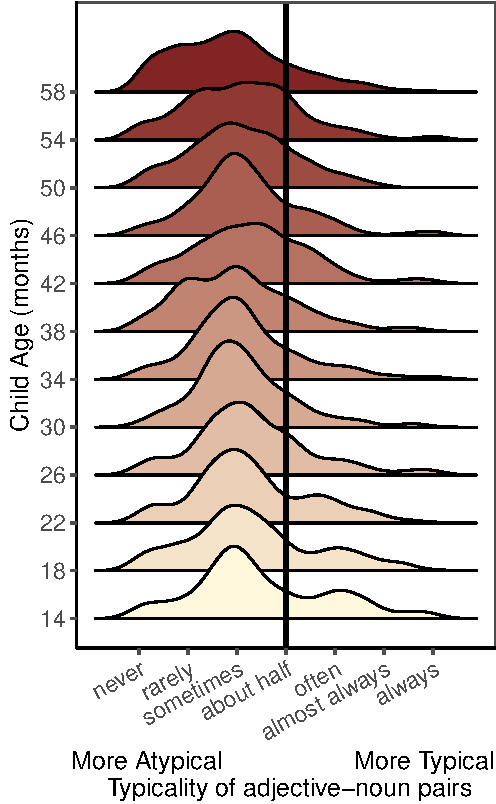
\includegraphics{figs/distribution_plot-1} 

}

\caption[Density plots showing usage at each timepoint based on the typicality of the adjective-noun pair]{Density plots showing usage at each timepoint based on the typicality of the adjective-noun pair.}\label{fig:distribution_plot}
\end{figure}
\end{CodeChunk}

To confirm this effect statistically, we centered the ratings (i.e.
``about half'' was coded as 0), and then predicted the rating on each
trial with a mixed effect model with only an intercept and a random
effect of noun (\texttt{typicality $\sim$ 1 + (1|noun)}). The intercept
was reliably negative, indicating that adjectives tend to refer to
atypical features of objects (\(\beta =\) -0.77, \(t =\) -19.72, \(p\)
\textless{} .001). We then re-estimated these models separately for each
age in the corpus, and found a reliably negative intercept for every age
group (smallest effect \(\beta_{14} =\) -0.5, \(t =\) -4.45, \(p =\)
\textless{} .001). These data suggest that even when talking with very
young children, caregiver speech is structured according to adult
communicative pressures observed in the lab.

For comparison, we performed the same analyses but with typicality
judgments weighted not by the frequency of each adjective-noun pair's
occurrence in the Language Development Project, but instead by their
frequency of occurrence in the Corpus of Contemporary American English
(COCA; Davies, 2008). While this estimate of adult usage is
imperfect---the adjective-nouns pairs produced by parents in our corpus
may not be a representative sample of adjectives and nouns spoken by the
adults in COCA---it provides a first approximation to adult usage. When
we fit the same mixed-effects model to the data, we found that the
intercept was reliably negative, indicating that adult-to-adult speech
is likely also biased toward description of atypical features
(\(\beta =\) -0.3, \(t =\) -19.72, \(p\) \textless{} .001)

Returning to caregiver speech, while descriptions at every age tended to
point out atypical features (as in adult-to-adult speech), this effect
changed in strength over development. An age effect added to the
previous model was reliably negative, indicating that parents of older
children are relatively more likely to focus on atypical features
(\(\beta =\) -0.11, \(t =\) -3.47, \(p =\) .001). In line with the idea
that caregivers adapt their speech to their children's knowledge, it
seems that caregivers are more likely to provide description of typical
features for their young children, compared with older children. As a
second test of this idea, we defined adjectives as highly typical if
Turkers judged them to be `often', `almost always', or `always' true. We
predicted whether each judgment was highly typical from a mixed-effects
logistic regression with a fixed effect of age (log-scaled) and a random
effect of noun. Age was a highly reliable predictor (\(\beta =\) -0.94,
\(t =\) -5.01, \(p =\) \textless{} .001). While children at all ages
hear more talk about what is atypically true (Figure
\ref{fig:distribution_plot}), younger children hear relatively more talk
about what is typically true than older children do (Figure
\ref{fig:prototypical_plot}).

\begin{CodeChunk}
\begin{figure}[tb]

{\centering 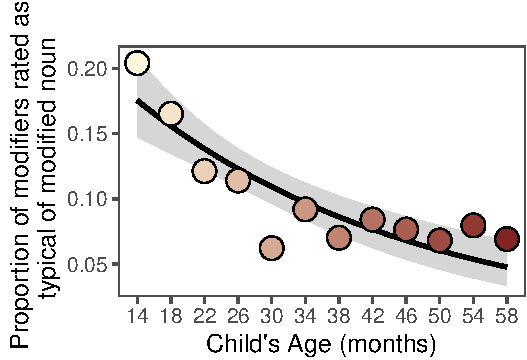
\includegraphics{figs/prototypical_plot-1} 

}

\caption[Proportion of caregiver description that is about typically-true features, as a function of age]{Proportion of caregiver description that is about typically-true features, as a function of age.}\label{fig:prototypical_plot}
\end{figure}
\end{CodeChunk}

\hypertarget{child-speech.}{%
\subsubsection{Child Speech.}\label{child-speech.}}

Given the striking consistency in adult-to-adult speech and caregiver
speech across ages, we next briefly consider what kind of information is
contained in children's speech. By analyzing children's own utterances,
we can determine when children come to use description in a way that
looks like adult speech. Are children mirroring adult-like uses of
description even from a young age, or are they choosing to describe more
typical features of the world?

The Language Development Corpus contains 368,348 child utterances. Using
the set of adjective-noun pairs for which we have judgments from our
analysis of caregiver speech, we repeat our analysis on usage data for a
set of 460 distinct adjective-noun pairs which also appeared in
children's productions. While preliminary, a mixed effects model
predicting typicality had a highly-reliable negative intercept
(\(\beta =\) -0.72, \(t =\) -10.14, \(p =\) \textless{} .001), but
adding an age term did not improve model fit. Thus, children's speech is
also biased towards atypical descriptions, and this bias does not change
reliably over the first 5 years.

\hypertarget{discussion}{%
\subsection{Discussion}\label{discussion}}

In sum, we find robust evidence that language is used to discuss
atypical, rather than typical, features of the world. Description in
caregiver speech seems to largely mirror the usage patterns that we
observed in adult-to-adult speech, suggesting that these patterns arise
from general communicative pressures. Indeed, even children's own
productions show a similar usage pattern, with more description of
atypical features of the world even at the youngest ages.

It should be noted that children's utterances come from naturalistic
conversations with caregivers, and their use of atypical description may
be prompted by parent-led discourse. That is, if a caregiver chooses to
describe the \emph{purpleness} of a cat in book, the child may well
respond by asking about that same feature. Further, atypical descriptors
may actually be more likely to elicit imitation from child speakers,
compared with typical descriptors (Bannard, Rosner, \& Matthews, 2017).
Future analyses would need to better disentangle the extent to which
children's productions are imitative of caregivers.

Interestingly, the descriptions children hear change over development,
becoming increasingly focused on atypical features. The higher
prevalence of typical descriptors in early development may help young
learners learn what is typical; however, even at the earliest point we
measured, the bulk of language input describes atypical features.

This usage pattern aligns with the idea that language is used
informatively in relation to background knowledge about the world. It
may pose a problem, however, for young language learners with
still-developing world knowledge. If language does not transparently
convey the typical features of objects, and instead (perhaps
misleadingly) notes the atypical ones, how might children come to learn
what objects are typically like? One possibility is that information
about typical features is captured in regularities across many
utterances. If this is true, language may still be an important source
of information about typicality as children may be able to extract more
accurate typicality information by tracking second-order co-occurrence.

\hypertarget{extracting-typicality-from-language-structure}{%
\section{Extracting Typicality from Language
Structure}\label{extracting-typicality-from-language-structure}}

Much information can be gleaned from language that does not seem
available at first glance. From language alone, simple distributional
learning models can recover enough information to perform comparably to
non-native college applicants on the Test of English as a Foreign
Language (Landauer \& Dumais, 1997). Recently, Lewis, Zettersten, \&
Lupyan (2019) demonstrated that even nuanced feature information may be
learnable through distributional semantics alone, without any complex
inferential machinery. We take a similar approach to ask whether a
distributional semantics model trained on the language children hear can
capture typical feature information.

\hypertarget{method}{%
\subsection{Method}\label{method}}

To test this possibility, we trained word2vec--a distributional
semantics model--on the same corpus of child-directed speech used in our
first set of analyses. Word2vec is a neural network model that learns to
predict words from the contexts in which they appear. This leads
word2vec to learn representations in which words that appear in similar
contexts become similar to each-other (Firth, 1957).

We used the continuous-bag-of-words (CBOW) implementation of word2vec in
the \texttt{gensim} package (Řehůřek \& Sojka, 2010). We trained the
model using a surrounding context of 5 words on either side of the
target word and 100 dimensions (weights in the hidden layer) to
represent each word. After training, we extracted the hidden layer
representation of each word in the model's vocabulary--these are the
vectors used to represent these words.

If the model captures information about the typical features of objects,
we should see that the model's noun-adjective word pair similarities are
correlated with the typicality ratings we elicited from human raters.
For a second comparison, we also used an off-the-shelf implementation of
word2vec trained on Wikipedia (Mikolov, Grave, Bojanowski, Puhrsch, \&
Joulin, 2018). While the Language Development Project corpus likely
underestimates the amount of structure in children's linguistic input,
Wikipedia likely overestimates it.

\hypertarget{results-1}{%
\subsection{Results}\label{results-1}}

We find that similarities in the model trained on the Language
Development Project corpus have near zero correlation with human
adjective--noun typicality ratings (\(r =\) 0.03, \(p =\) .208).
However, our model does capture other meaningful information about the
structure of language, such as similarity. Comparing with pre-existing
large-scale human similarity judgements for word pairs, our model shows
significant correlations (correlation with wordsim353 similarities of
noun pairs, 0.28; correlation with simlex similarities of noun,
adjective, and verb pairs, 0.16). This suggests that statistical
patterns in child-directed speech are likely insufficient to encode
information about the typical features of objects, despite encoding at
least some information about word meaning more broadly.

However, the corpus on which we trained this model was small; perhaps
our model did not get enough language to draw out the patterns that
would reflect the typical features of objects. To test this possibility,
we asked whether word vectors trained on a much larger corpus---English
Wikipedia---strongly correlate with typicality ratings. This model's
similarities were significantly correlated with human judgments,
although the strength of the correlation was still fairly weak (\(r =\)
0.25, \(p\) \textless{} .001). Interestingly, similarities from the two
models correlated more highly to each other than either model correlated
with human judgments (\(r =\) 0.29, \(p\) \textless{} .001). This
suggests that these models are picking up on some systematic
associations between nouns and adjectives, but not the typical features
of things.

One possible confound in these analyses is that the similarity judgments
produced by our models reflect many dimensions of similarity, but our
human judgments reflect only typicality. To accommodate this, we
performed a second analysis in which we considered only the subset of 73
nouns that had both a typical (rated as at least ``often'') and an
atypical (rated as at most ``sometimes'') adjective. We then asked
whether the models rated the typical adjective as more similar to the
noun it modified than the atypical adjective. The LDP model correctly
classified 38 out of 73 (0.52), which was not better than chance
(\(p =\) .815). The Wikipedia model correctly classified 56 out of 73
(0.77), which was better than chance according to a binomial test, but
still fairly poor performance (\(p =\) \textless{} .001). Fig
\ref{fig:halfs} shows the ratings from Turkers and the two models for
the 73 nouns. Table \ref{tab:pairs_tab} gives the six cases in which
word2vec similarities are worst at predicting human typicality
judgments, judging the low-typicality adjective to be \emph{more}
similar to the noun than the high-typicality adjective.

\begin{CodeChunk}
\begin{figure}[tb]

{\centering \includegraphics{figs/halfs-1} 

}

\caption[Plots of word2vec noun-adjective similarities for nouns for which there was at least one atypical adjective (rated at most "sometimes"), and at least one typical adjective (rated at least "often")]{Plots of word2vec noun-adjective similarities for nouns for which there was at least one atypical adjective (rated at most "sometimes"), and at least one typical adjective (rated at least "often").}\label{fig:halfs}
\end{figure}
\end{CodeChunk}

\begin{table}[tb]
\centering
\begin{tabular}{lll}
  \hline
noun & typical adjective & atypical adjective \\ 
  \hline
puzzle & flat & giant \\ 
  apple & red & brown \\ 
  bird & outside & purple \\ 
  elephant & fat & pink \\ 
  whale & wet & red \\ 
  frog & green & purple \\ 
   \hline
\end{tabular}
\caption{The top six cases in which Wikipedia-trained word2vec similarities were worst at predicting human typicality judgments. In each case, word2vec judged the low-typicality adjective to be more similar to the noun than the high-typicality adjective.} 
\label{tab:pairs_tab}
\end{table}

\hypertarget{general-discussion}{%
\section{General Discussion}\label{general-discussion}}

Language provides children a rich source of information about the world.
However, this information is not always transparently available: because
language is used to comment on the atypical, it does not perfectly
mirror the world. Among adult conversational partners whose world
knowledge is well-aligned, this allows people to converse informatively
and avoid redundancy. But between a child and caregiver whose world
knowledge is asymmetric, this pressure competes with other demands: what
is minimally informative to an adult may be misleading to a child. Our
results show that this pressure structures language to create a peculiar
learning environment, one in which caregivers predominantly point out
the atypical features of things.

How, then, do children learn about the typical features of things? While
younger children may gain an important foothold from hearing more
description of typical features, they still face language dominated by
atypical description. When we looked at more nuanced ways of extracting
information from language (which may or may not be available to the
developing learner), we found that models of distributional semantics
capture little typical feature information.

Of course, perceptual information from the world may simplify this
problem. In many cases, perceptual information may swamp information
from language; children likely see enough orange carrots in the world to
outweigh hearing ``purple carrot.'' It remains unclear, however, how
children learn about categories for which they have scarcer evidence.
Indeed, language information likely swamps perceptual information for
many other categories, such as abstract concepts or those that cannot be
learned about by direct experience. If such concepts pattern similarly
to the concrete objects analyzed here, children are in a particularly
difficult bind.

It is also possible that other cues from language and interaction
provide young learners with clues to what is typical or atypical, and
these cues are uncaptured by our measure of usage statistics. Caregivers
may highlight when a feature is typical by using certain syntactic
constructions, such as generics (e.g., ``tomatoes are red''). Caregivers
may also mark the atypicality of a feature, for example demonstrating
surprise. Such cues from language and the interaction may provide key
information in some cases; however, given the sheer frequency of
atypical descriptors, it seems unlikely that they are consistently
well-marked.

Another possibility is that children expect language to be used
informatively at a young age. Under this hypothesis, their language
environment is not misleading at all, even without additional cues from
caregivers. Children as young as two years old tend to use words to
comment on what is new rather than what is known or assumed (Baker \&
Greenfield, 1988). Children may therefore expect adjectives to comment
on surprising features of objects. If young children expect adjectives
to mark atypical features (Horowitz \& Frank, 2016), they can use
description and the lack thereof to learn more about the world. Indeed,
this idea is consistent with our finding that even young children
largely choose to describe atypical features. Though this effect can be
explained by simpler means such as mimicry, it suggests that caregivers
and children may be usefully aligned in the aspects of the world they
choose to talk about.

Whether adult-directed, child-directed, or a child's own speech,
language is used with remarkable consistency: people talk about the
atypical. Though parents might reasonably be broadly over-informative in
order to teach their children about the world, this is not the case.
This presents a potential puzzle for young learners who have limited
world knowledge and limited pragmatic inferential abilities. Perceptual
information and nascent pragmatic abilities may help fill in the gaps,
but much remains to be explored to link these explanations to actual
learning. Communication pressures are pervasive forces structuring the
language children hear, and future work must disentangle whether
children capitalize on them or are misled by them in learning about the
world.

\vspace{1em} \fbox{\parbox[b][][c]{7.3cm}{\centering Stimuli, data, and analysis code available at\ \url{https://osf.io/ypdzv/}}}

\hypertarget{acknowledgements}{%
\section{Acknowledgements}\label{acknowledgements}}

This research was funded by a James S. McDonnell Foundation Scholar
Award to DY.

\hypertarget{references}{%
\section{References}\label{references}}

\setlength{\parindent}{-0.1in} 
\setlength{\leftskip}{0.125in}

\noindent

\hypertarget{refs}{}
\leavevmode\hypertarget{ref-baillargeon1994}{}%
Baillargeon, R. (1994). How do infants learn about the physical world?
\emph{Current Directions in Psychological Science}, \emph{3}(5),
133--140.

\leavevmode\hypertarget{ref-baker1988}{}%
Baker, N. D., \& Greenfield, P. M. (1988). The development of new and
old information in young children's early language. \emph{Language
Sciences}, \emph{10}(1), 3--34.

\leavevmode\hypertarget{ref-bannard2017}{}%
Bannard, C., Rosner, M., \& Matthews, D. (2017). What's worth talking
about? Information theory reveals how children balance informativeness
and ease of production. \emph{Psychological Science}, \emph{28}(7),
954--966.

\leavevmode\hypertarget{ref-bedny2019}{}%
Bedny, M., Koster-Hale, J., Elli, G., Yazzolino, L., \& Saxe, R. (2019).
There's more to ``sparkle'' than meets the eye: Knowledge of vision and
light verbs among congenitally blind and sighted individuals.
\emph{Cognition}, \emph{189}, 105--115.

\leavevmode\hypertarget{ref-brysbaert2014}{}%
Brysbaert, M., Warriner, A. B., \& Kuperman, V. (2014). Concreteness
ratings for 40 thousand generally known english word lemmas.
\emph{Behavior Research Methods}, \emph{46}(3), 904--911.

\leavevmode\hypertarget{ref-davies2008}{}%
Davies, M. (2008). The corpus of contemporary american english (coca):
520 million words, 1990-present.

\leavevmode\hypertarget{ref-firth1957}{}%
Firth, J. R. (1957). A synopsis of linguistic theory, 1930-1955.
\emph{Studies in Linguistic Analysis}.

\leavevmode\hypertarget{ref-goldin-meadow2014}{}%
Goldin-Meadow, S., Levine, S. C., Hedges, L. V., Huttenlocher, J.,
Raudenbush, S. W., \& Small, S. L. (2014). New evidence about language
and cognitive development based on a longitudinal study: Hypotheses for
intervention. \emph{American Psychologist}, \emph{69}(6), 588.

\leavevmode\hypertarget{ref-grice1975}{}%
Grice, H. P. (1975). Logic and conversation. In \emph{Speech acts} (pp.
41--58). Brill.

\leavevmode\hypertarget{ref-harris2006}{}%
Harris, P. L., \& Koenig, M. A. (2006). Trust in testimony: How children
learn about science and religion. \emph{Child Development},
\emph{77}(3), 505--524.

\leavevmode\hypertarget{ref-horowitz2016}{}%
Horowitz, A. C., \& Frank, M. C. (2016). Children's pragmatic inferences
as a route for learning about the world. \emph{Child Development},
\emph{87}(3), 807--819.

\leavevmode\hypertarget{ref-johns2012}{}%
Johns, B. T., \& Jones, M. N. (2012). Perceptual inference through
global lexical similarity. \emph{Topics in Cognitive Science},
\emph{4}(1), 103--120.

\leavevmode\hypertarget{ref-landau2009}{}%
Landau, B., Gleitman, L. R., \& Landau, B. (2009). \emph{Language and
experience: Evidence from the blind child} (Vol. 8). Harvard University
Press.

\leavevmode\hypertarget{ref-landauer1997}{}%
Landauer, T. K., \& Dumais, S. T. (1997). A solution to plato's problem:
The latent semantic analysis theory of acquisition, induction, and
representation of knowledge. \emph{Psychological Review}, \emph{104}(2),
211.

\leavevmode\hypertarget{ref-legare2016}{}%
Legare, C. H., \& Harris, P. L. (2016). The ontogeny of cultural
learning. \emph{Child Development}, \emph{87}(3), 633--642.

\leavevmode\hypertarget{ref-lewis2019}{}%
Lewis, M., Zettersten, M., \& Lupyan, G. (2019). Distributional
semantics as a source of visual knowledge. \emph{Proceedings of the
National Academy of Sciences}, \emph{116}(39), 19237--19238.

\leavevmode\hypertarget{ref-mikolov2018}{}%
Mikolov, T., Grave, E., Bojanowski, P., Puhrsch, C., \& Joulin, A.
(2018). Advances in pre-training distributed word representations. In
\emph{Proceedings of the international conference on language resources
and evaluation (lrec 2018)}.

\leavevmode\hypertarget{ref-mikolov2013}{}%
Mikolov, T., Sutskever, I., Chen, K., Corrado, G. S., \& Dean, J.
(2013). Distributed representations of words and phrases and their
compositionality. In \emph{Advances in neural information processing
systems} (pp. 3111--3119).

\leavevmode\hypertarget{ref-rhodes2012}{}%
Rhodes, M., Leslie, S.-J., \& Tworek, C. M. (2012). Cultural
transmission of social essentialism. \emph{Proceedings of the National
Academy of Sciences}, \emph{109}(34), 13526--13531.

\leavevmode\hypertarget{ref-rogers2004}{}%
Rogers, T. T., \& McClelland, J. L. (2004). \emph{Semantic cognition: A
parallel distributed processing approach}. MIT press.

\leavevmode\hypertarget{ref-rubio-fernandez2016}{}%
Rubio-Fernández, P. (2016). How Redundant Are Redundant Color
Adjectives? An Efficiency-Based Analysis of Color Overspecification.
\emph{Frontiers in Psychology}, \emph{7}.

\leavevmode\hypertarget{ref-rehurek2010}{}%
Řehůřek, R., \& Sojka, P. (2010). Software Framework for Topic Modelling
with Large Corpora. In \emph{Proceedings of the LREC 2010 Workshop on
New Challenges for NLP Frameworks} (pp. 45--50). Valletta, Malta: ELRA.

\leavevmode\hypertarget{ref-sloutsky2004}{}%
Sloutsky, V. M., \& Fisher, A. V. (2004). Induction and categorization
in young children: A similarity-based model. \emph{Journal of
Experimental Psychology: General}, \emph{133}(2), 166.

\leavevmode\hypertarget{ref-snow1972}{}%
Snow, C. E. (1972). Mothers' speech to children learning language.
\emph{Child Development}, 549--565.

\leavevmode\hypertarget{ref-stahl2015}{}%
Stahl, A. E., \& Feigenson, L. (2015). Observing the unexpected enhances
infants' learning and exploration. \emph{Science}, \emph{348}(6230),
91--94.

\leavevmode\hypertarget{ref-westerbeek2015}{}%
Westerbeek, H., Koolen, R., \& Maes, A. (2015). Stored object knowledge
and the production of referring expressions: The case of color
typicality. \emph{Frontiers in Psychology}, \emph{6}.

\leavevmode\hypertarget{ref-willits2008}{}%
Willits, J. A., Sussman, R. S., \& Amato, M. S. (2008). Event knowledge
vs. Verb knowledge. In \emph{Proceedings of the 30th annual conference
of the cognitive science society} (pp. 2227--2232).

\bibliographystyle{apacite}


\end{document}
